\section{Struttura del File JSON per la Definizione di una Rete Bayesiana}\label{strutturaRete}

Questa sezione ha lo scopo di spiegare all'utente il corretto modo di definire il file \textit{.JSON} per la definizione della rete bayesiana da importare nel plug-in e successivamente utilizzala.


\begin{figure}[H]
	\begin{center}
		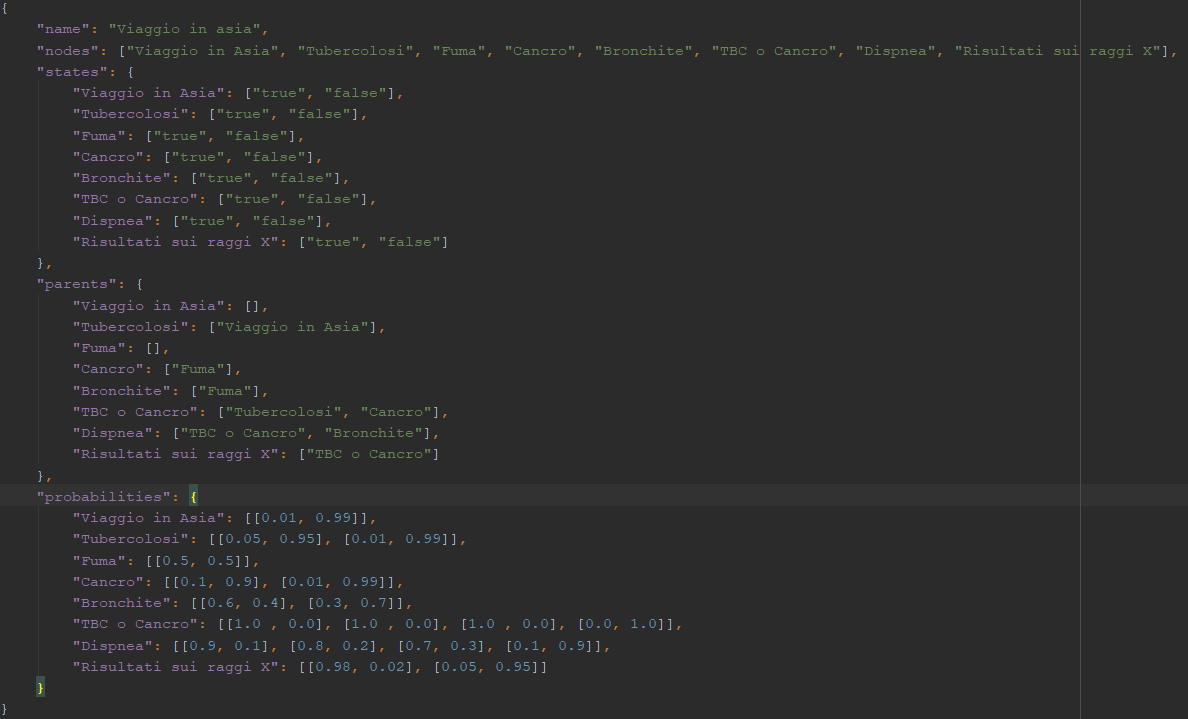
\includegraphics[scale=0.6]{./images/strutturaRete.png}
		 \caption{Rete Bayesiana Correttamente Definita}	
		 \label{ImgRete}
	\end{center}
\end{figure}

Passi da seguire :
\begin{itemize}
 \item Il file \textit{.JSON} dovrà contenere 5 campi più esterni, denominati:
 	\begin{itemize}
 		\item name;
 		\item nodes;
 		\item states;
 		\item parents;
 		\item probabilities.
 	\end{itemize}
 	I nomi dei campi devono iniziare con la lettera minuscola corrispondente. Qualora uno dei campi non abbia il nome corretto come sopra, verrà visualizzato il seguente errore (nel seguente caso mancava il campo name, sostituito da un nome non valido): 
 	\begin{figure}[H]
	\begin{center}
		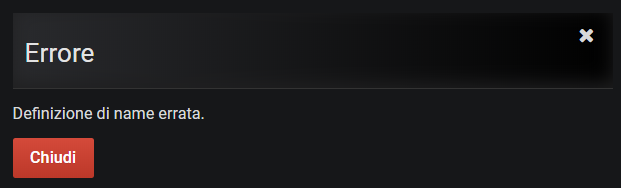
\includegraphics[scale=0.6]{./images/erroreNomeCampo.png}
		 \caption{Errore nel Nome di un Campo della Rete Bayesiana}	
		 \label{ImgRete}
	\end{center}
\end{figure}

	Se viene inserito un numero errato di campi diverso da 5, verrà visualizzato il seguente errore:
	
	\begin{figure}[H]
	\begin{center}
		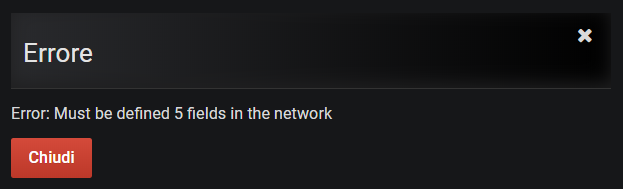
\includegraphics[scale=0.6]{./images/wrongNumberOfFields.png}
		 \caption{Errore Numero di Campi della Rete Errato}	
		 \label{ImgRete}
	\end{center}
\end{figure}

	\item Il campo successivo dovrà chiamarsi nodes e dovrà contenere un array, nel quale sono definiti i nomi dei nodi della rete bayesiana.\label{nomi} I campi states, parents e probabilities, dovranno ognuno contenere al proprio interno un numero di campi pari al numero di nomi definiti nel campo nodes e con lo stesso nome. Qualora sia definito all'interno di uno di essi un numero errato di campi, verrà visualizzato il seguente errore (ad esempio se manca un nome in states): 

\begin{figure}[H]
	\begin{center}
		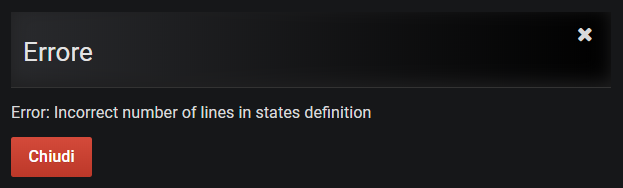
\includegraphics[scale=0.6]{./images/numberFields.png}
		 \caption{Errore Numero di Campi}	
		 \label{erNumCampi}
	\end{center}
\end{figure}

Se invece il numero di campi è giusto ma non viene trovato uno dei nomi in nodes, verrà visualizzato il seguente errore ( il nodo tubercolosi è stato sostituito con un nome non valido):

\begin{figure}[H]
	\begin{center}
		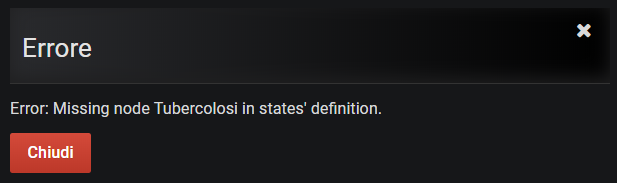
\includegraphics[scale=0.6]{./images/wrongName.png}
		 \caption{Errore Nome di un Campo Interno}	
		 \label{erNumCampi}
	\end{center}
\end{figure}

	\item Il campo successivo dovrà chiamarsi states e dovrà essere composto nel seguente modo:
	\begin{itemize}
		\item Deve rispettare quanto detto  in \ref{nomi};
		\item Ogni campo dovrà contenere un array con almeno 2 valori al suo interno, altrimenti verrà visualizzato il seguente errore :
		
		\begin{figure}[H]
	\begin{center}
		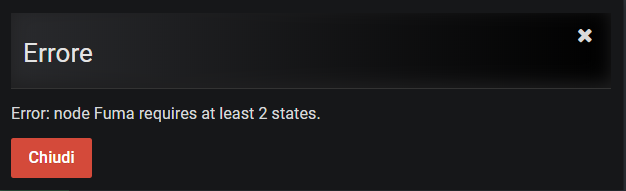
\includegraphics[scale=0.6]{./images/twoStates.png}
		 \caption{Errore Nodo con Meno di 2 Stati}	
		 \label{erTwoStates}
	\end{center}
	\end{figure}
	
		\item Uno stato non può essere ripetuto, altrimenti verrà visualizzato il seguente errore:
	\end{itemize}
	
	\begin{figure}[H]
	\begin{center}
		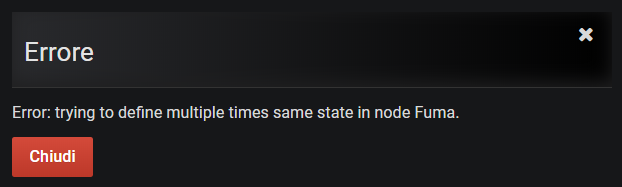
\includegraphics[scale=0.6]{./images/multipleState.png}
		 \caption{Errore Stato Ripetuto}	
		 \label{erMultipleState}
	\end{center}
	\end{figure}
	
	\item Il campo successivo dovrà chiamarsi parents e dovrà essere composto nel seguente modo:
	
	\begin{itemize}
		\item Deve rispettare quanto detto  in \ref{nomi};
		\item Ogni campo dovrà contenere un array, nel quale si possono inserire i padri del nodo qualora ne abbia;
		\item I padri devono essere nomi contenuti nel campo nodes, altrimenti verrà visualizzato il seguente errore ( inserito un padre chiamato notValid ):
		
	\begin{figure}[H]
	\begin{center}
		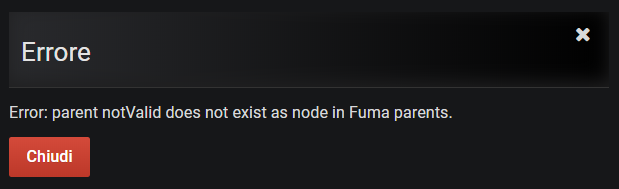
\includegraphics[scale=0.6]{./images/unexistingNode.png}
		 \caption{Errore Padre non Esistente}	
		 \label{erUnexistingNode}
	\end{center}
	\end{figure}	
	
	\item Un nodo non può essere definito come padre di se stesso, altrimenti verrà visualizzato il seguente errore ( fuma definito come padre di se stesso ):	
	
	\begin{figure}[H]
	\begin{center}
		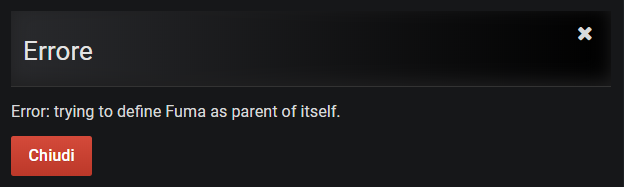
\includegraphics[scale=0.6]{./images/padreDiSeStesso.png}
		 \caption{Errore Padre di Sé Stesso}	
		 \label{erUnexistingNode}
	\end{center}
	\end{figure}	
	
	\item Non è possibile definire più volte lo stesso padre per un nodo, altrimenti verrà visualizzato il seguente errore (Fuma definito 2 volte come padre per tubercolosi ): 
	
	\begin{figure}[H]
	\begin{center}
		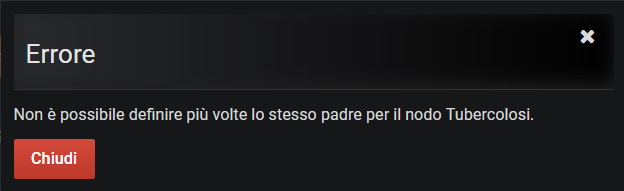
\includegraphics[scale=0.6]{./images/padreRipetuto.png}
		 \caption{Errore Padre Ripetuto}	
		 \label{erUnexistingNode}
	\end{center}
	\end{figure}	
		
	\end{itemize}
	
	\item Il campo successivo dovrà chiamarsi probabilities e dovrà essere composto nel seguente modo:
	
	\begin{itemize}
		\item Deve rispettare quanto detto  in \ref{nomi};
		\item Ogni campo deve contenere un array, contenente a sua volta tanti sotto-array pari alla produttoria del numero di stati di ogni padre del nodo, in caso contrario verrà visualizzato il seguente errore(3 al posto di 4):
		
		\begin{figure}[H]
	\begin{center}
		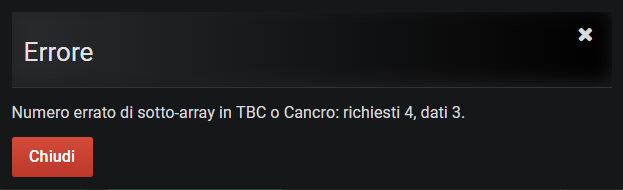
\includegraphics[scale=0.6]{./images/wrongSubsets.png}
		 \caption{Errore Numero di Subset}	
		 \label{erWrongSubsets}
	\end{center}
	\end{figure}	
		
		\item Ogni sotto-array deve contenere un numero di valori pari al numero di stati del nodo, in caso contrario verrà visualizzato il seguente errore(3 al posto di 2): 
		
		\begin{figure}[H]
	\begin{center}
		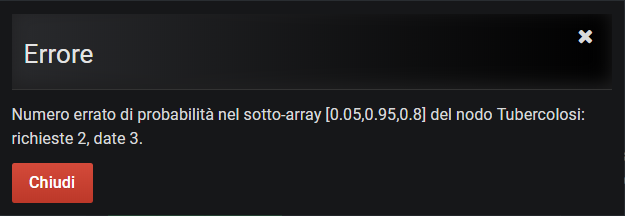
\includegraphics[scale=0.6]{./images/numberProbs.png}
		 \caption{Errore Numero di Probabilità nel Sotto-array}	
		 \label{erWrongSubsets}
	\end{center}
	\end{figure}	
	
	\item Le probabilità devono essere numeri compresi tra 0 e 1, altrimenti verrà visualizzato il seguente errore(probabilità = 5):
	
	\begin{figure}[H]
	\begin{center}
		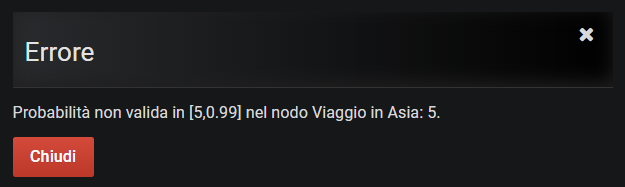
\includegraphics[scale=0.6]{./images/invalidProbability.png}
		 \caption{Errore Probabilità non Valida}	
		 \label{erWrongSubsets}
	\end{center}
	\end{figure}
		
	\end{itemize}
	
	\item Le probabilità vanno inserite nel seguente modo:
	 \begin{itemize}
	 		\item in ogni sotto-array le probabilità vanno inserite in ordine in base a come sono stati definiti gli stati del nodo, quindi come in figura \ref{ImgRete} la probabilità 0.01 verrà associata allo stato true e la probabilità 0.99 verrà associata allo stato false;
	 		\item I sotto-array vanno a definire le probabilità condizionate dai padri, e vanno messi in ordine, quindi ad esempio in figura \ref{ImgRete} per il nodo TBC o Cancro, il primo sotto-array andrà a definire le probabilità per p("TBC o Cancro" | Tubercolosi = true, Cancro = true), il secondo p("TBC o Cancro" | Tubercolosi = true, Cancro = false), il terzo p("TBC o Cancro" | Tubercolosi = false, Cancro = true) e l'ultimo p("TBC o Cancro" | Tubercolosi = false, Cancro = false), quindi in ordine secondo come sono stati definiti gli stati dei padri. Nel caso in cui si sbagli a definire i sotto-array, rispettando però i punti precedenti, non verrà visualizzato un errore ma i calcoli non rispetteranno quanto atteso.
	 \end{itemize}
	
	
	
	
	
	
	
	
	

\end{itemize}